\documentclass[border=5mm,tikz]{standalone} 

\usepackage{amsmath}
% !TEX root=img/arguments_and_attack.tex

% \usetikzlibrary{external} 
% \tikzexternalize[prefix=tikz/] 

\usetikzlibrary{calc}
\usetikzlibrary{arrows}
\usetikzlibrary{arrows.meta}
\usetikzlibrary{decorations.markings}
% \usetikzlibrary{intersections}
\usetikzlibrary{fit}
\usetikzlibrary{shapes}
% \usetikzlibrary{trees}


\tikzset{
	every path/.style={thick},
	align=center,
	observed/.style={
		fill=black!20,
	},
	bn/.style={
		draw,
		ellipse,
		-{Triangle[angle=60:6pt 0]}
	},
	scn/.style={
		draw,
		rectangle,
		% signal,
		% signal from=west,
		% signal pointer angle=120,
		-{Triangle[angle=60:6pt 0]},
	},
	possibly/.style={dashed},
	arg/.style={
		draw,
		rectangle,
		-{Straight Barb[angle=60:6pt 0]}
	},
	attack/.style={
		-{Rays[width=10pt,length=10pt,sep=-3.9pt]}
	},
	subscn/.style={
		double,
		-{Triangle[angle=60:6pt 0]},
	},
	specific/.style={
		double,
		-{Stealth[angle=60:6pt 0]}
	},
}



\begin{document}
	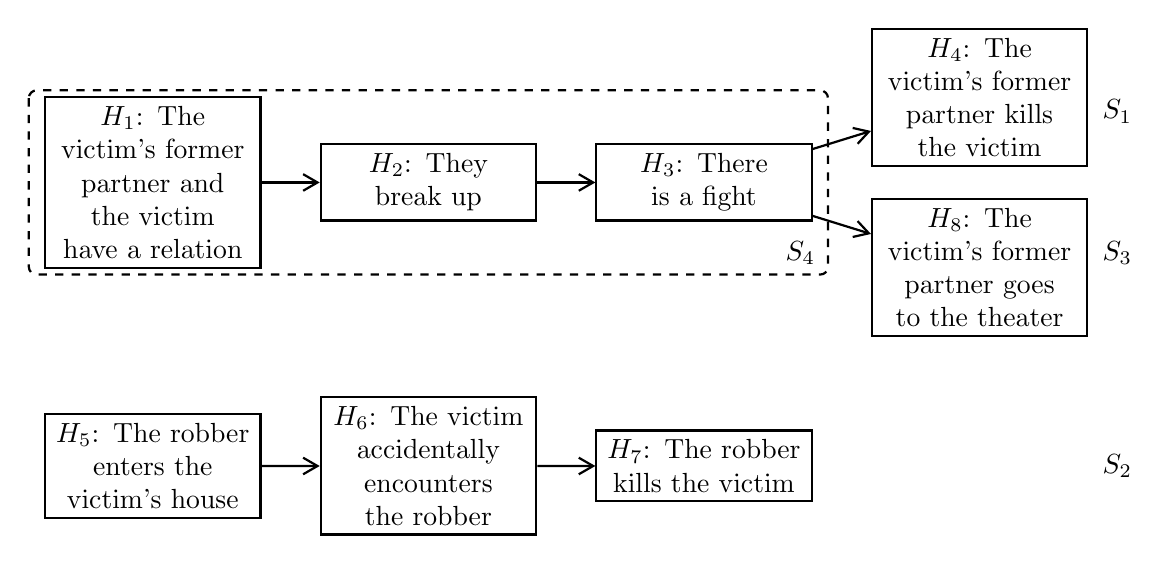
\begin{tikzpicture}[
		scn/.append style={text width=2.5cm},
		arg/.append style={text width=3cm},
	]
		\pgftransformxscale{3.5}
		\pgftransformyscale{1.8}
		
		\node[scn] (H1) at (1,0) {$H_1$: The victim's former partner and the victim have a relation};
		\node[scn] (H2) at (2,0) {$H_2$: They break up};
		\node[scn] (H3) at (3,0) {$H_3$: There is a fight};

		\node[scn] (H4) at (4,0.6) {$H_4$: The victim's former partner kills the victim};

		\node at (4.5,0.5) {$S_1$};

		\node[scn] (H8) at (4,-0.6) {$H_8$: The victim's former partner goes to the theater};

		\node at (4.5,-0.5) {$S_3$};

		\node[scn] (H5) at (1,-2) {$H_5$: The robber enters the victim's house};
		\node[scn] (H6) at (2,-2) {$H_6$: The victim accidentally encounters the robber};
		\node[scn] (H7) at (3,-2) {$H_7$: The robber kills the victim};

		\node at (4.5,-2) {$S_2$};

		\draw[thick,dashed,rounded corners=1mm] (0.55,0.65) rectangle (3.45,-0.65);
		\node at (3.35,-0.5) {$S_4$};

		\draw[arg] (H1) -- (H2);
		\draw[arg] (H2) -- (H3);
		\draw[arg] (H3) -- (H4);
		\draw[arg] (H3) -- (H8);
		\draw[arg] (H5) -- (H6);
		\draw[arg] (H6) -- (H7);


	\end{tikzpicture}
\end{document}
